% Read the readme first!
% options:
% - uulm-draft: show todonotes, links, linenumbers hide label names
% - uulm-draft-verbose: show todonotes, links, linenumbers, label names
% - uulm-release-electronic: show links, hide todonotes, linenumbers, label names
% - uulm-release-print hide everything
%
\documentclass[uulm-release-print]{thesis-uulm}

% workarround for some stupid error in combination with IEEEtran, bibtex and babel.
\makeatletter
\def\markboth#1#2{%
  \def\leftmark{\@IEEEcompsoconly{\sffamily}#1}%
  \def\rightmark{\@IEEEcompsoconly{\sffamily}#2}}
\makeatother

% create vectors
\usepackage{amsmath}
\usepackage{subfigure}

% Choose language
%%\usepackage[ngerman]{babel}
 \usepackage[english]{babel}

% Fonts
\renewcommand{\sfdefault}{phv}
\renewcommand{\rmdefault}{phv}
\renewcommand{\ttdefault}{pcr}

% Adjust variables
\author{Marco Combosch}
\title{An In-Depth Analysis of and Compensation for the Heisenberg Effect}
\email{marco.combosch@uni-ulm.de}
\matnr{868772}	% Student ID
\degree{Media Informatics} %program you are enrolled

\type{Bachelor Thesis} % Type of Thesis (Bachelors, Masters)
\jahr{2019}

\gutachterA{Prof. Dr. Enrico Rukzio} % First Reviewer
%\gutachterB{Prof. Dr. Un Leserlich}  % Second reviewer
\betreuer{Dennis Wolf} % supervisor

% Can be user to only compile parts of the document
\includeonly{
template/definitions,
chapters/introduction,
chapters/related-work,
chapters/content,
chapters/evaluation,
chapters/conclusion,
chapters/appendix
}

% Definitions for code listings
%% definitions.tex
%%

%Listings für die Darstellung der Treiber im Anhang:
%-------------------------------------------------------
\usepackage{listings}

\usepackage{color}
\definecolor{gray}{rgb}{0.4,0.4,0.4}
\definecolor{darkblue}{rgb}{0.0,0.0,0.6}
\definecolor{cyan}{rgb}{0.0,0.6,0.6}

\lstset{
  basicstyle=\ttfamily,
  columns=fullflexible,
  showstringspaces=false,
  commentstyle=\color{gray}\upshape
}

\lstdefinelanguage{XML}
{
  morestring=[b]",
  morestring=[s]{>}{<},
  morecomment=[s]{<?}{?>},
  stringstyle=\color{black},
  identifierstyle=\color{darkblue},
  keywordstyle=\color{cyan},
  morekeywords={xmlns,version,type}% list your attributes here
}
%-----------------------------------------------------------


\begin{document}

\frontmatter %%%%%%%%%%%%%%%%%%%%%%%%%%%%%%%%%%%%%%%%%%%%%%%%%%%%%%%%%%%%%%%%%
\pagenumbering{roman}
\begin{nolinenumbers}
\maketitle

\copyrightpage
\end{nolinenumbers}

\setstretch{1.2}

\begin{abstract}

In modern virtual reality (VR) systems, distal interaction with a controller on canvas is the standard input model. In games and applications in VR, distal pointing is used as the main interface to interact with the virtual environment. Some of them need precise selections to work accurately. Predictable and accurate pointing can also reduce frustration when working and/or playing in VR. Some scientific papers suggest that the ``Heisenberg Effect'', an effect resulting in selecting a target by clicking or pressing a button, has an impact on the performance, accuracy and usability of VR applications. This thesis takes a look at this ``Heisenberg Effect'', it's underlying mechanism and on possible actions to compensate the effect. The foundation of this work is a study which was implemented to analyze if the ``Heisenberg Effect'' can be detected and what its effect is. 

The evaluation of the collected data suggests, that the ``Heisenberg Effect'' exists and has an impact on accuracy and performance on distal pointing tasks. On the basis of this statement, a short overview of ideas is given, on how to compensate this effect. These ideas give a basis for future work on this topic.

\end{abstract}

\begin{nolinenumbers}
\tableofcontents
\end{nolinenumbers}

\mainmatter %%%%%%%%%%%%%%%%%%%%%%%%%%%%%%%%%%%%%%%%%%%%%%%%%%%%%%%%%%%%%%%%%%
\pagenumbering{arabic}
%% introduction.tex
%%
\chapter{Introduction}
\label{ch:introduction}

\section{Pointing in VR}

In normal desktop applications, the mouse is the standard device for input. Mobile devices use mostly touchscreens and sometimes gyroscopes as input devices, where the mouse and the touchscreen or -pad work on a 2D plane. 

In contrast to that, virtual reality (VR) uses pointing in three dimensions to present the applications and to receive inputs. Most modern VR devices use a controller with three (3DOF) or six (6DOF) degrees of freedom to navigate and select in the virtual environment (VE). 

The actions are based on the procedure of the user pointing the controller to the desired target and selecting the target by clicking or pressing a button on the controller. Sometimes this pointing is indicated in VR by a raycast. This raycast shows the direction and the aim of the position of the controller, by spawning a ray out of the top of the device. The user has then the opportunity to directly see, where he's pointing with the controller. Because the controller is tracked in at least three dimensions, the action of selecting something (by clicking or pressing) has an impact on the position of the controller itself, and therefore on the resulting position of the selection on the canvas. This unintentional change of the selected position by selecting something is described in some scientific papers as the ``Heisenberg Effect''.

This paper gives an in-depth view on this ``Heisenberg Effect'', shows its impact and what actions are required to compensate it. To show the ``Heisenberg Effect'', it's required to isolate other effects, caused by the three dimensional (3D) architecture of the VR controller and the virtual environment. 

Based on this it is necessary to understand these effects and to take note of these effects in investigating the ``Heisenberg Effect''.

\section{Objective}

Applications in VR rely on a dependable interaction with the user. To gain immersion, it is necessary, that a user has the sense, the virtual environment correctly responds to his actions. If selections and clicks are not registered by the system, caused by different effects, immersion suffers from this experience. One of these effects could be the so-called ``Heisenberg Effect''. Because it is only referenced in a small amount of scientific papers, more research on this topic is needed. To understand this ``Heisenberg Effect'' better and even show it's impact is incentive for this thesis. Finding a way to compensate the effect is also one of the motives for this work because reliable selections are the basis for good and efficient user experience.

\section{Structure}

To have a good insight into the topic of distal pointing and the associated effects, this work takes at first a look at related work in the field of distal pointing. Used procedures for study design and to analyze these effects are also described in the second chapter (Related Work -~\ref{ch:related-work}). To have a good basis on describing and characterizing the ``Heisenberg Effect'' a short view on the already done work will be a part of the second chapter. 

To explore more aspects of this effect, a study was carried out. The third chapter (Content -~\ref{ch:content}) takes a look on the way of implementing a useful study design, and the used resources and algorithms. The experiment is explained in detail and a short look on the resulted data is given.

The collected data out of the experiment is analyzed and discussed in the fourth chapter (Results -~\ref{ch:results}). Also, an explanation of the ``Heisenberg Effect'' based on this data is given. The last chapter (Conclusions and future work -~\ref{ch:conclusion}) takes a look on the now newly described ``Heisenberg Effect'' and shows some steps that could compensate this effect. Incentives and lookouts for future work on this topic are also presented.
%% related-work.tex
%%

\chapter{Related Work}
\label{ch:related-work}

The ``Heisenberg Effect'' is described only in a few scientific papers. First mentioned in the paper by Bowman et al.~\cite{bowman_using_2001}, and picked up by Kopper et al~\cite{kopper_human_2010}, a real definition and evidence for the ``Heisenberg Effect'' were never given. In this section, a general definition, based on the previous works mentioned before, is drawn up and explained. To analyze and describe the Heisenberg Effect it is necessary to take a look at different researches on pointing tasks and the used procedures. Therefore, a detailed look at related work on 2D and 3D pointing tasks, spatial jitter, and resulting effects is given. Based on these papers this chapter is concluded by taking a look at underlying laws and algorithms which are used in the later study design to show and analyze the ``Heisenberg Effect''.

\section{Defining the Heisenberg Effect}
\label{sec:related-work:defining-heisenberg-effect}

\subsection{First reference by Bowman et al.}
\label{subsec:related-work:defining-heisenberg-effect:first-reference}

The first reference of the ``Heisenberg Effect'' was in the paper ``Using Pinch Gloves\textsuperscript{TM} for both Natural and Abstract Interaction Techniques in Virtual Environments'' by Bowman et al.~\cite{bowman_using_2001}. The paper shows the use of cloth gloves (called after the brand name ``Pinch Gloves\textsuperscript{TM}'') as input devices in virtual environments. They also describe different techniques to interact in VR with these gloves.  One problem they mentioned in their paper, was the difficulty to point at an object and simultaneously select it, without disturbing the previous pointing. This effect was called ``the Heisenberg Effect of spatial interaction''. To avoid this ``Heisenberg Effect'' while still using the selected gloves, they used one hand to point to the desired target and then the other hand to select it. More pieces of information or hints are not given by the mentioned paper. The meaning of the name ``Heisenberg Effect'' could be derived by ``Heisenberg's uncertainty principle'' in physics, declare it is only possible to either point on something with certainty or to select something with certainty. But not both at the same time.

\subsection{Description and link to Fitt's Law by Kopper et al.}
\label{subsec:related-work:defining-heisenberg-effect:description}

The term ``Heisenberg Effect'' was also used in the work of Kopper et al.~\cite{kopper_human_2010} called ``A human motor behavior model for distal pointing tasks''. This paper takes a focus on distal pointing tasks and gives an overview of different models to precisely measure movement time, by extending Fitt's Law. They conclude, that the natural hand jitter and the movement made while pressing down a button to select a target, add to an increase in movement time and difficulty. They call this effect also ``Heisenberg Effect'' and refer to the work of Bowman et al.~\cite{bowman_using_2001}.

\subsection{Own definition}
\label{subsec:related-work:defining-heisenberg-effect:definition}

Based on the previous work by Bowman and Kopper, the ``Heisenberg Effect'' in this thesis is defined as follows:

\begin{quote}
The ``Heisenberg Effect in distal pointing'' describes the difference between the position of a mental selection of a target and the real tracked position, distinguished by the disturbance of the selecting action.
\end{quote}

To show the ``Heisenberg Effect'' in an example, a look at Figure~\ref{fig:heisenberg_effect} shows a 
scenario, where a user is pointing with a controller via raycast on a target. The line P1 describes the acquired direction and aim of the user right before he is selecting the target by pressing or clicking a button. Trough the action of select the target, the raycast gets disturbed which is shown exemplarily by line P2. The now arising difference between ``wanted position'' and ``resulted position'' on the canvas is what was described previously and called the ``Heisenberg Effect'' (labeled as H1).

\begin{figure}[h]
    \centering
    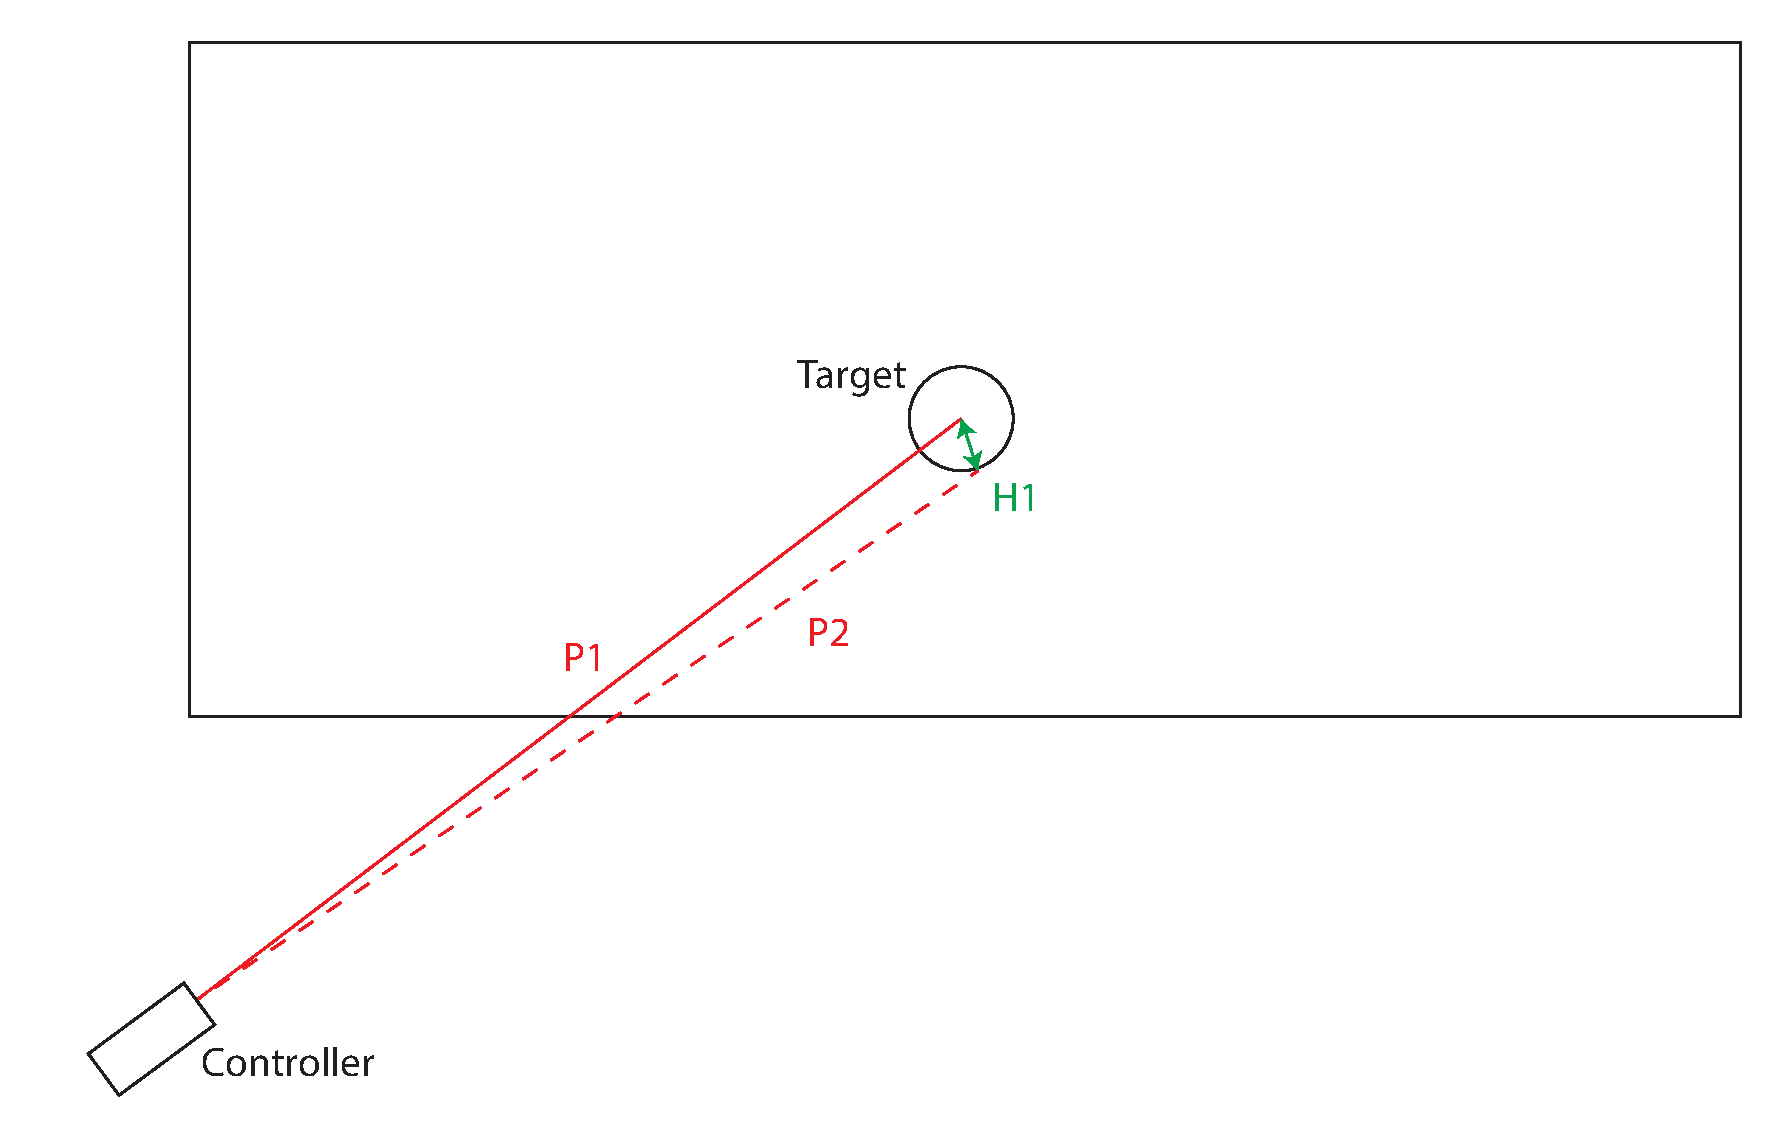
\includegraphics[width=.9\columnwidth]{graphics/heisenberg_effect.pdf}
    \caption{Describing the Heisenberg Effect on a simple distal pointing task example}
    \label{fig:heisenberg_effect}
\end{figure}

Based on this definition, this thesis wants to show, that the ``Heisenberg Effect'' exists, can be measured and therefore compensated.

\section{Background \& Related Work on pointing tasks}
\label{sec:related-work:pointion-tasks}

\subsection{Distal pointing tasks}

To measure and analyze accuracy in distal pointing, many studies use distal pointing tasks. In Figure~\ref{fig:pointing_task} a simple setup of such a task is shown. In VR the user handles with a controller a visible ray cast. This ray cast is a ray emitted from the tip of the controller in the given direction controlled by the user. If this ray cast hits a canvas the user can see, on which target on the canvas he points his controller (the ray cast is in Figure~\ref{fig:pointing_task} the red line P1). With a button on the controller, the user can select now a target on the canvas on which he is pointing at the moment he presses or clicks the button. In a distal pointing task, target after target is shown to the user and he has to move his controller in the direction of the target and select it with a press/click on the button.
These movements can be analyzed and described by Fitt's Law:

\subsection{Fitts' Law}
\label{subsec:related-work:background:fitts_law}

Fitts' Law is a model to calculate movement times and the difficulties of movements between a start point and a target or between two targets. The difficulty of such movements, called Index of Difficulty (\textit{ID}) and measured in bits, is described in one-dimension as:

\[\ ID = \log_2 (2 \cdot A / W) \]

where \textit{A} is the distance (or amplitude) between two targets and \textit{W} is the size of the target. In this work we use for \textit{ID} the so called ``Shannon formulation'' as suggested by MacKenzie and Buxton~\cite{mackenzie_extending_1992}, to scale on two-dimensions, fit better the observation and correct negative values for \textit{ID}:

\[ ID = \log_2 (A / W + 1) \]

\newpage

 Based on this Index of Difficulty, Fitts' Law describes the Movement Time (\textit{MT}) as follows:

\[ MT = a + b \cdot ID\]

a and b are empirically determined constant values based on the given input devices for the specific pointing task. Fitt's Law argues by these equations, that correct movements to targets get more difficult if the targets get smaller. With movement time (\textit{MT}) and \textit{ID}, we can calculate the throughput of an input device in bits per second:

\[ TP = ID / MT \]

\subsection{Extended Fitt's Law}
\label{subsec:related-work:background:extended_fitts_law}

In the study design for this work an extended model of the Fitt's Law, proposed by MacKenzie~\cite{mackenzie_fitts_law_reasearch_tool} and described on pointing tasks by Kong and Ren~\cite{kong_calculation_2006}, is used. MacKenzie claims in his paper, that the traditional Fitt's Law doesn't account the actual performance of a user when trying to hit small targets. For the extended
%Groß/Klein
Fitt's Law used here, the values for Distance and Width (now called \textit{Effective Distance} and \textit{Effective Width}) are calculated for the set of collected data. By using the standard deviation, the extended Fitt's Law can filter out different strategies used by the user to accomplish the tasks. MacKenzie described the \textit{Effective Witdh} as follows:

\[ W_e = 4.133 \cdot \sigma \]

where $\sigma$ is the standard deviation defined as:

\[ \sigma = \frac{\sum_{i=1}^{n} (x_i - \bar{x}) }{\sqrt{n - 1}}  \]

where $n$ is the number of trials and the sum describes the sum of deviations. As in the standard Fitt's Law the \textit{Effective Throughput} is defined here as:

\[ TP_e = \frac{ID_e}{MT_{mean}} \]

where 

\[ ID_e = \log_2 (\frac{A_e}{W_e} + 1) \]

\subsection{Related work on distal pointing}
\label{subsec:related-work:background:realted_work_on_distal_pointing}

The extended Fitt's Law is used in the work done by alternately Pavlovych, Stuerzlinger, MacKenzie and Teather~\cite{pavlovych_tradeoff_2009}~\cite{teather_effects_2009}~\cite{teather_pointing_2011} to analyze the effects of spatial jitter and lag on the performance in distal pointing tasks. Spatial jitter is described by Pavlovych and Stuerzlinger~\cite{pavlovych_tradeoff_2009} as ``a combination of hand tremor and noise in the device signal''. Their work gave a good foundation for the study design of this paper, mainly because of three reasons:

\begin{itemize}
    \item The study design in all three papers used the ISO 9241-9 specification~\cite{douglas_testing_1999} which gives clear conditions for this study design. Although the specification was not fully applied.
    \item To isolate the ``Heisenberg Effect'', it was important to clear our data from disturbances like the effects of hand tremor and noises of the device signals, described in their work.
    \item To give further works a base on how the ``Heisenberg Effect'' may affect performance in distal pointing tasks, by taking a look on the \textit{Effective Troughput} proposed by MacKenzie.
\end{itemize}





%% content.tex
%%
\chapter{Content}
\label{ch:content}

To show the ``Heisenberg Effect'' a study design based on the work done by Pavlovych and Stuerzlinger~\cite{pavlovych_tradeoff_2009} was set up. The foundation of the study was a simple distal pointing task. This section gives an insight into the underlying implementation and considerations for the used study design. The experiment and the procedure are also described in detail. 

\section{Implementation}
\label{sec:implementation}

\subsection{Setup}
\label{subsec:impl:setup}

For the study, it was used the HTC Vive PRO and Unity with Steam VR to create the study setup. The controller for the HTC Vive PRO has a trigger at the bottom to click and select targets. To stay near the real devices, this trigger was used as the main button. The implementation is described in detail in the next sections. Based on the environment with Unity, C\# was used as the main programming language.
In the room in which the study was performed, it was built up two tracking sensors, to capture most of the room. In the center of the room stood a chair, fixed on the ground. An HTC Vive Pro headset and one controller were used in the demonstration. The user stood on the predefined spot in front of the chair or sit on it. 

\subsection{First attempts}
\label{subsec:impl:first_attempts}

The goal of the study was to find possible effects and evidence for the ``Heisenberg Effect''. As the effect described in a previous section (Subsection~\ref{subsec:related-work:defining-heisenberg-effect:description}), it was necessary to create a point and aim application for measuring the overall movements and hits, performed by the study subjects. Even at the beginning of implementation, it was clear to collect data of clicks out of the movement and in a static position. The aim of these two scenarios was to find and show differences in clicks out of motion and resting clicks (the clicks out of motion were discarded because of too many disturbances). Resulting from this specification, it was created a procedure for a single target task:

\newpage

\begin{enumerate}
    \item Show one target
    \item Wait for first click (not necessarily on target) - arising out of the movement
    \item Show counter if the user is on target and wait for the counter to finish
    \item Wait for second click (also not necessarily on target)
    \item Hide the target and begin again with the next one
\end{enumerate}

With this specification, it was possible to observe differences in static and motion-based clicks. This specification was transferred into the final implementation.
\newline
\newline
After solving the problem of the procedure, it was necessary to clarify how to arrange the targets on the canvas. The first attempt in implementation was to show a grid-based target layout (as shown in Figure~\ref{fig:layout-attempts} (a)).

\begin{figure}[h]
    \centering
    \subfigure[First layout attempt with grid based layout]{{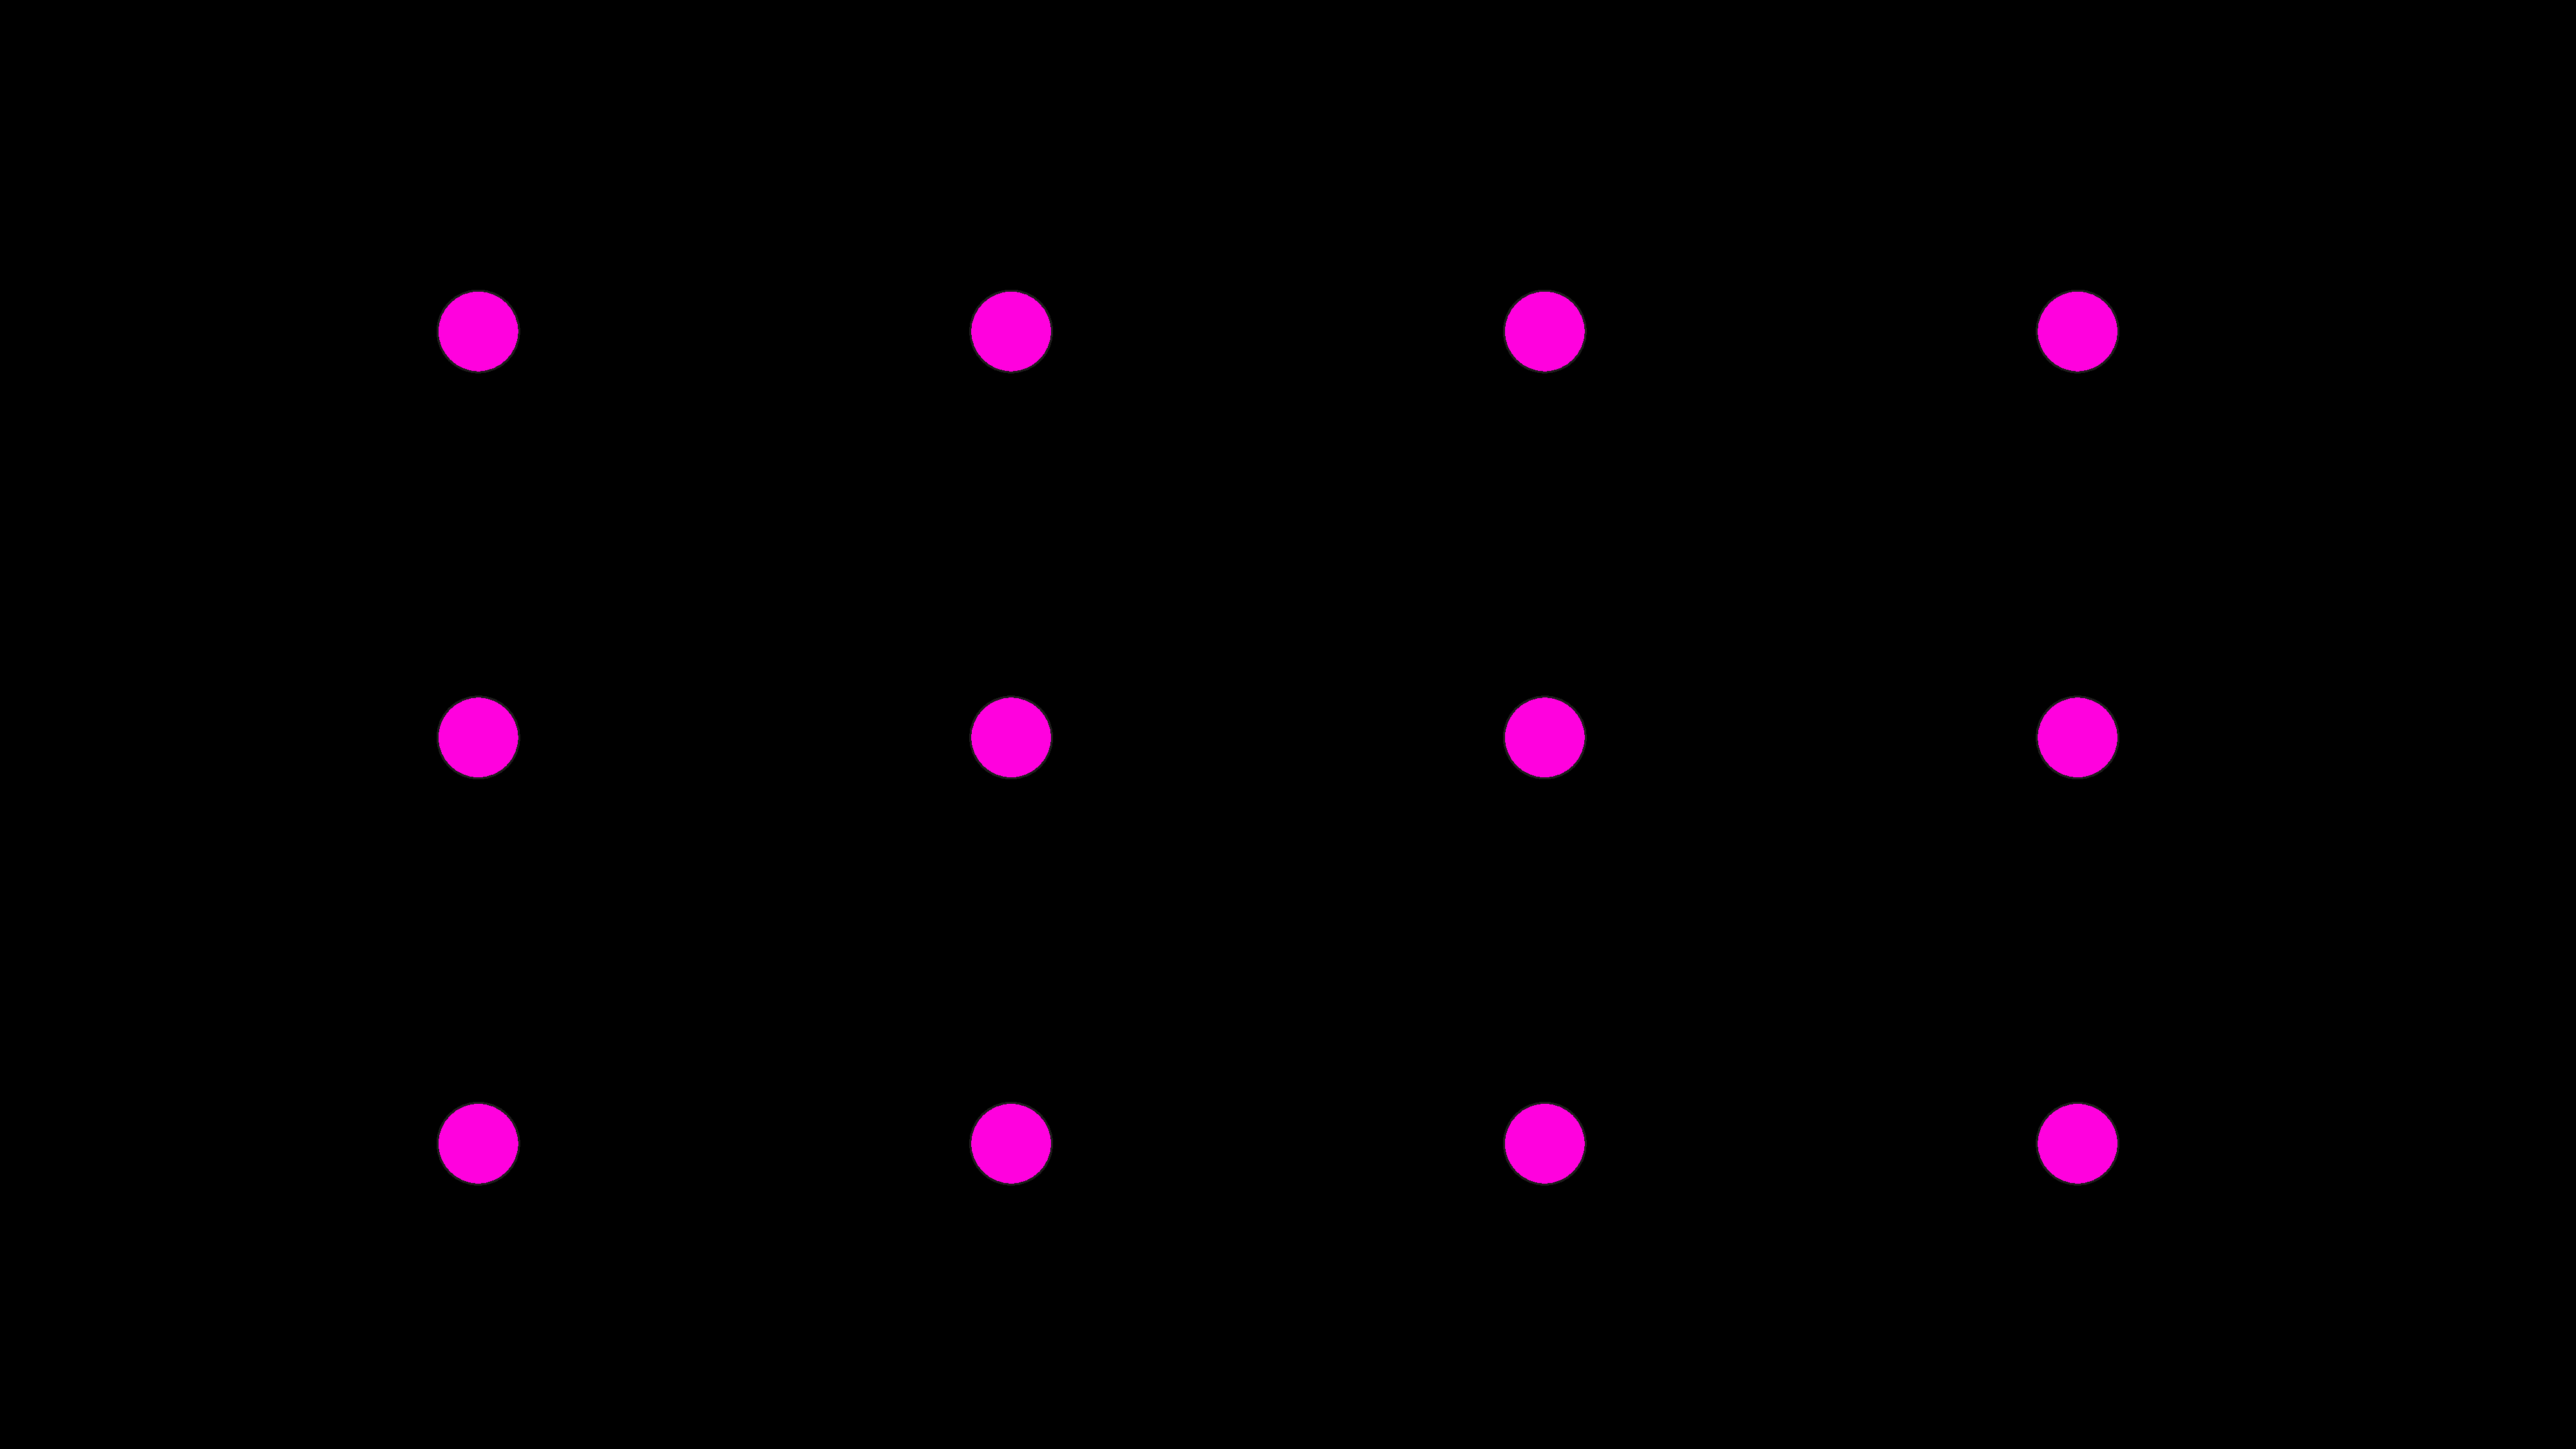
\includegraphics[width=.4\linewidth]{graphics/grid.pdf}}}
    \qquad
    \subfigure[Grid based attempt in first implementation. After finishing the trial (with only three targets) the result is shown (the green points show the position of the raycast when the user clicked.)]{{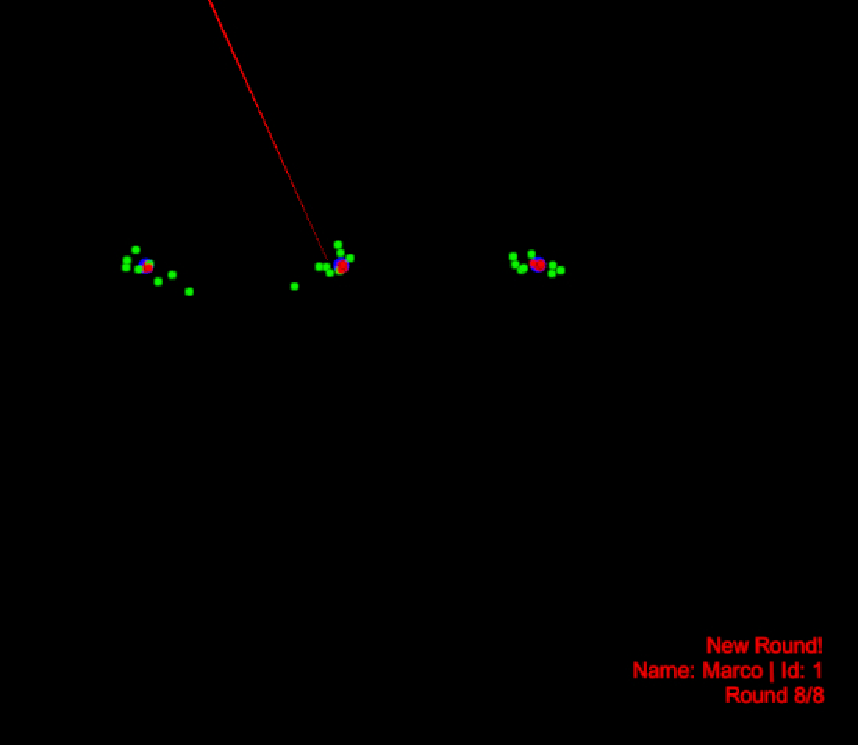
\includegraphics[width=.5\linewidth]{graphics/in_app_graphics/heisenberg_before_end_small.pdf}}}
    \caption{Different Layout attempts}
    \label{fig:layout-attempts}
\end{figure}

The targets were displayed, one after another, on a three-by-four grid (three in height and four in width). Depending on the grid layout, there were three possible ways to display the targets one after another: 

\begin{enumerate}
    \item Show them in a static order
    \item Show them in a random order
    \item Create different static orders and rotate through them randomly
\end{enumerate}

The first layouts and experiments were based on this grid. After some testing (one of the results of the test runs is shown in Figure~\ref{fig:layout-attempts} (b)), there were some issues with this type of grid layout: The distances between the targets were different, caused by the three-by-four grid. Also, no other studies used such a grid layout for testing accuracy in pointing tasks. After some research, the paper by Pavlovych and Stuerzlinger~\cite{pavlovych_tradeoff_2009} showed some usable target layout. They used a Fitts' Law based circle task to test accuracy in their pointing tasks, which was adopted to this setup (see ~\ref{subsec:impl:circle_task}).
\newline

Based on the used setup (\ref{subsec:impl:setup}), the software should also handle most of the functionality the controller and the system supported. The controller supported six degrees of freedom (free position in three dimensions, plus three-dimensional angles). To portray also results for controllers with three degrees of freedom (fixed position, but three-dimensional angles), a mode for switching between these variations was implemented. 

The controller uses a  trigger to measure clicks. These clicks are not binary, meaning the strength of a press on the trigger can be measured by decimal values between 0.0 (trigger not touched) and 1.0 (trigger fully pressed). In the implementation, these values get also tracked to see, when a user initialized the click by slightly pressing the trigger, and when the click is really registered as a click by the implementation.

Besides the mode for degrees of freedom, the implementation handles two different modes, to create more variety in the study setup. The position of the user's arm (stretched out or applied to the body) and the position of the user itself (standing or sitting) is also tracked.

\begin{figure}[h]
    \centering
    \subfigure[Circle layout (the user was shown only one target at a time)]{{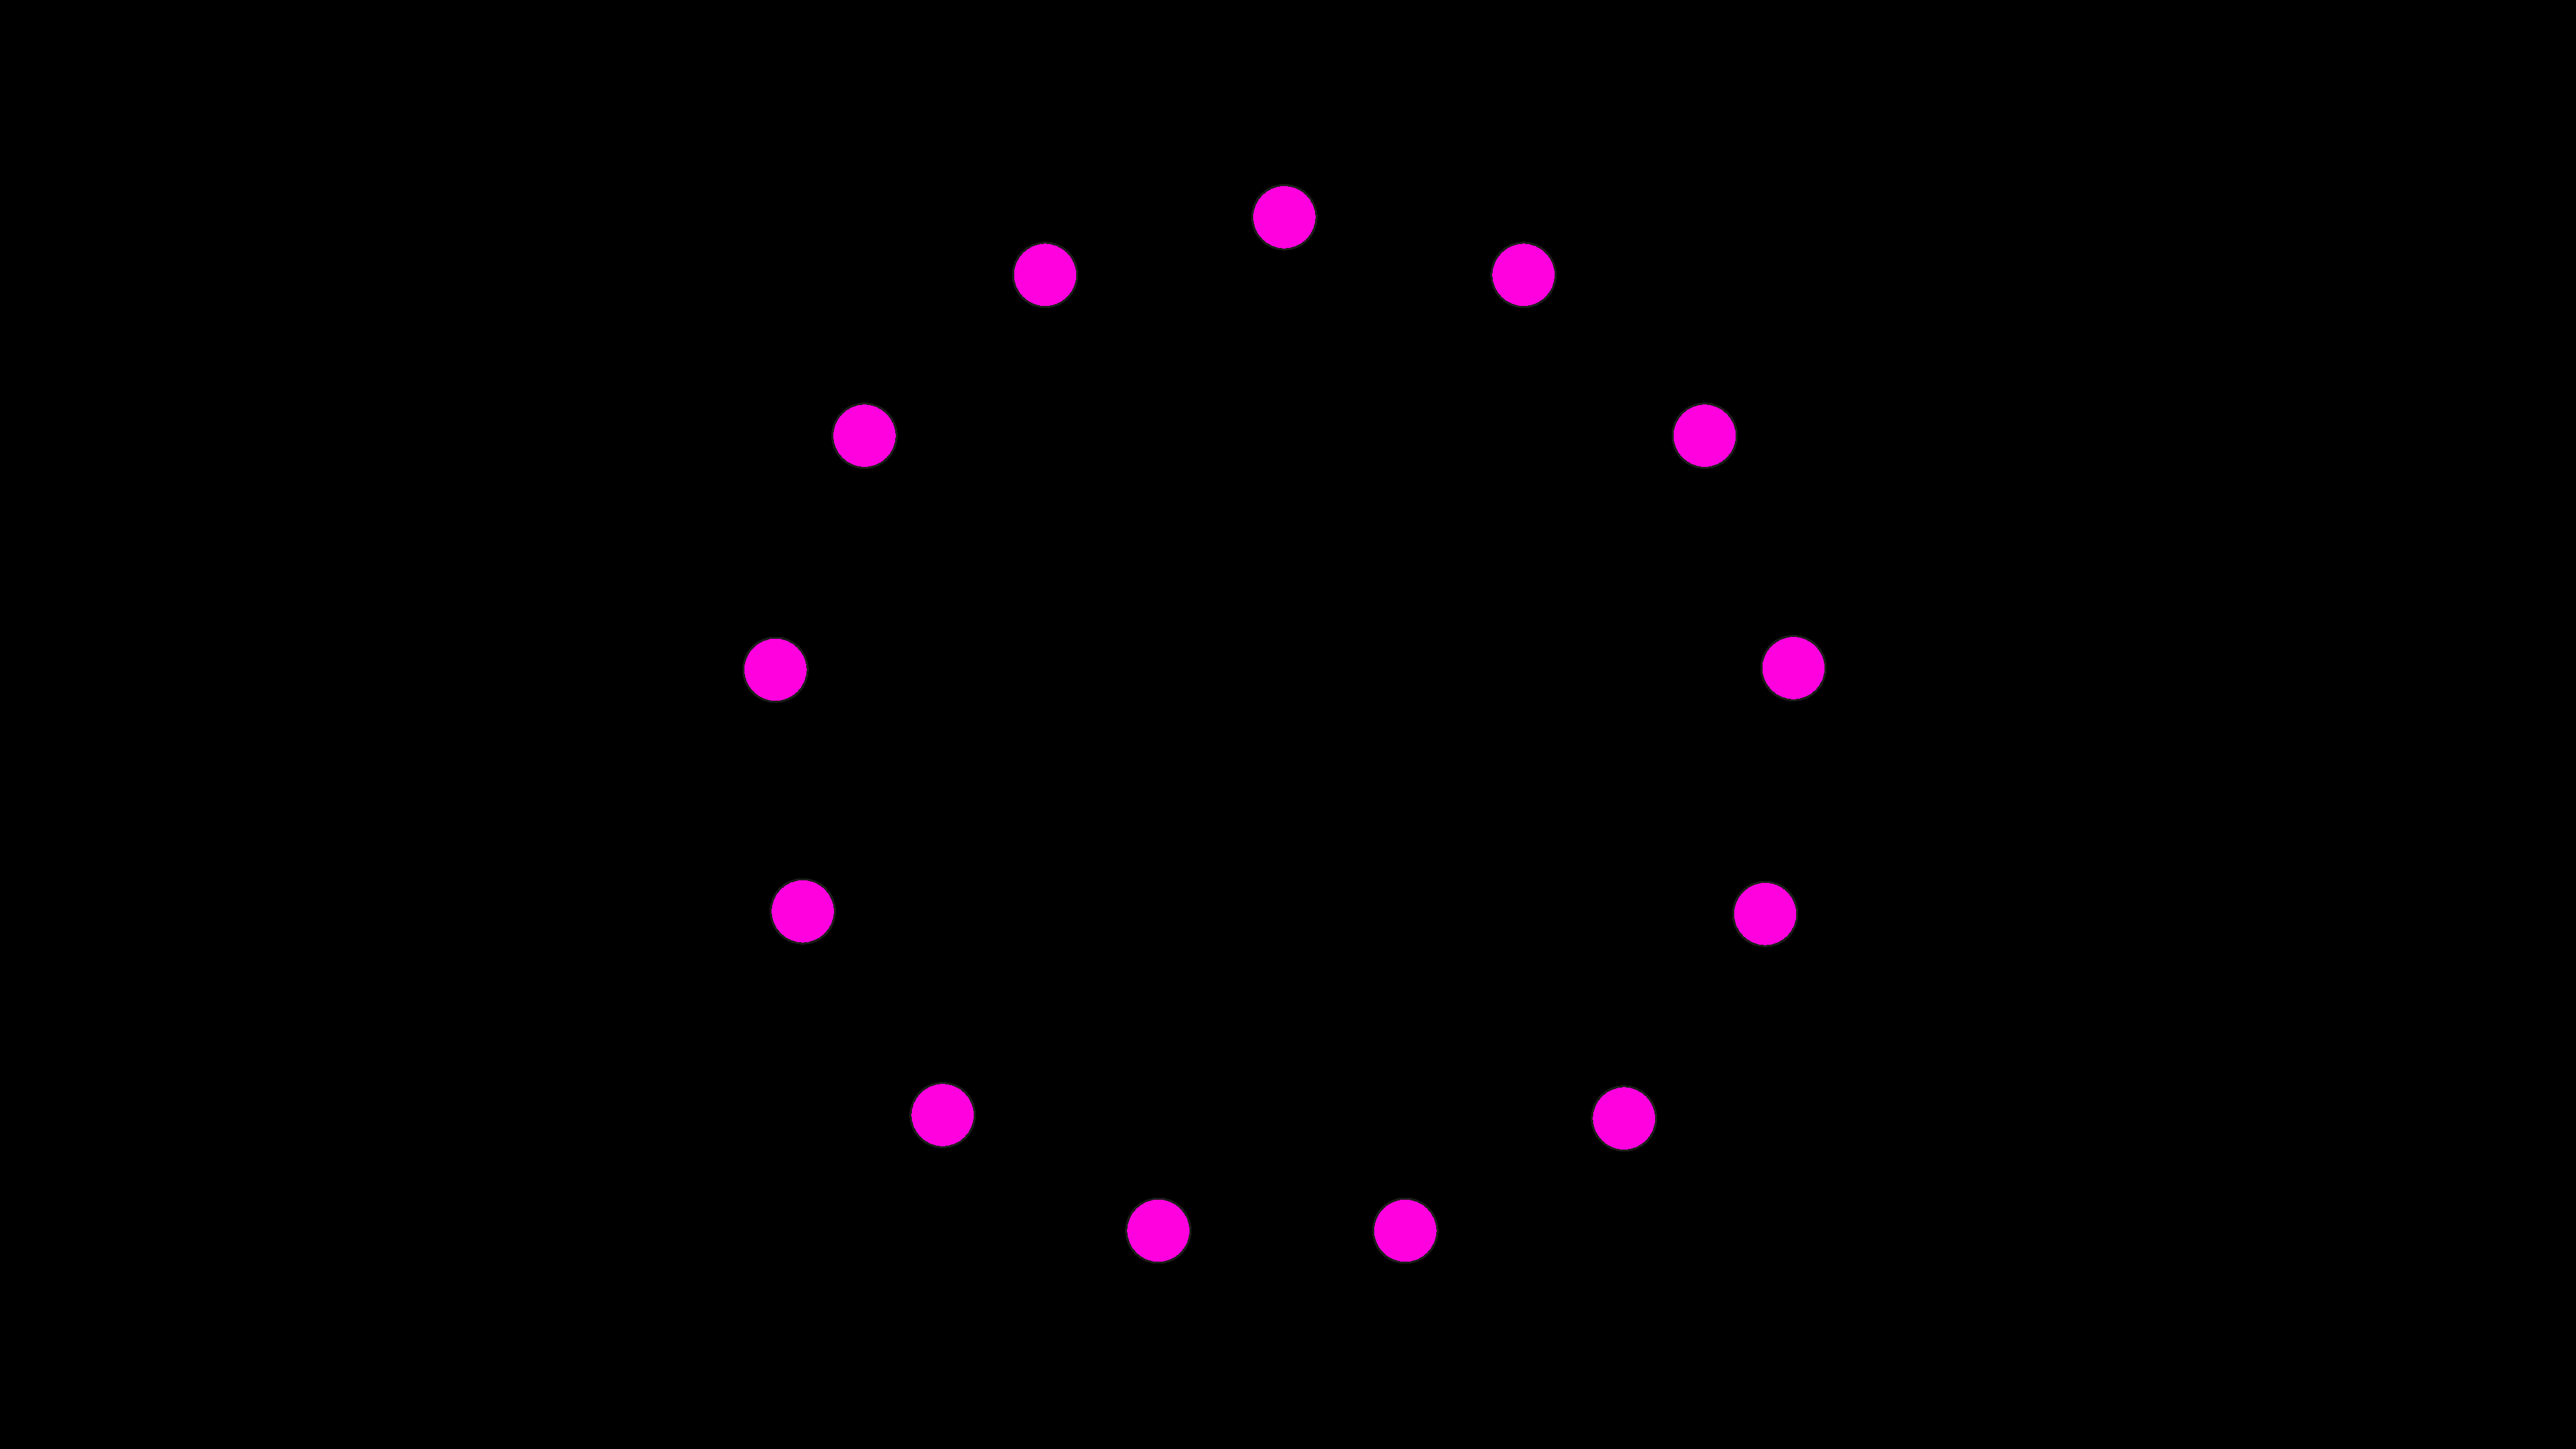
\includegraphics[width=.4\linewidth]{graphics/fitts_law_circle_in_app.pdf}}}
    \qquad
    \subfigure[Single target in real application]{{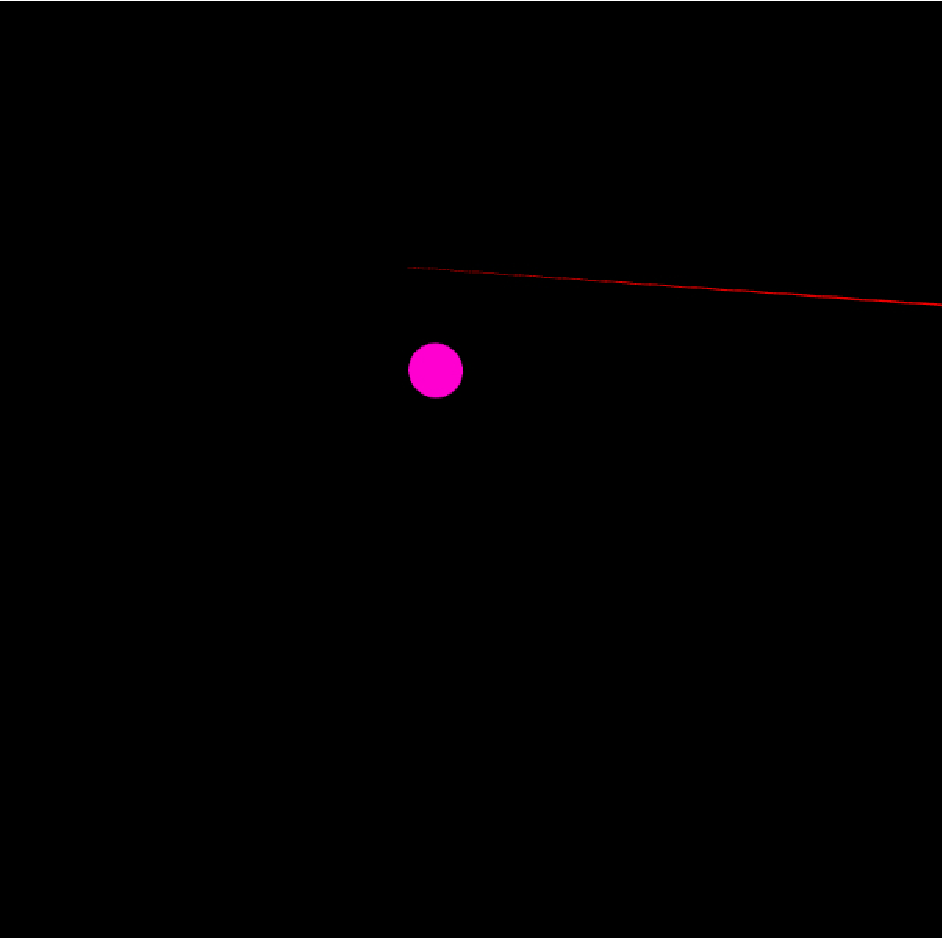
\includegraphics[width=.5\linewidth]{graphics/in_app_graphics/heisenberg_final_click_small.pdf}}}
    \caption{Final implementation}
    \label{fig:layout-final-implementation}
\end{figure}

\begin{table}
    \centering
    \begin{tabular}{c | c | c}
    \toprule
    Width & Amplitude & ID \\
    \midrule
    15  & 150   & 3.46 \\
    15  & 350   & 4.60 \\
    30 & 150 & 2.58 \\
    30 & 350 & 3.66 \\
    50 & 150 & 2.00 \\
    50 & 350 & 3.00
    \end{tabular}
    \caption{Used Index of Difficulty}
    \label{tab:id_values}
\end{table}

\subsection{Fitts' Law based circle pointing task}
\label{subsec:impl:circle_task}

Based on the experience made with a grid-base pointing task (described in section above: ~\ref{subsec:impl:first_attempts}), it was clear to use a Fitts' Law based circle pointing task as described by Soukoreff and MacKenzie~\cite{soukoreff_towards_2004}. To get a wide range of difficulties in the study, the \textit{ID} was calculated with different numbers of \textit{Amplitude} and \textit{Width} to get diverse \textit{ID}'s as described in Table~\ref{tab:id_values}.

On the basis of the \textit{Width} and \textit{Amplitude} values, described in Table~\ref{tab:id_values} for each \textit{ID} value was created an own Fitts' Law based circle pointing task.  In consideration of the study setup by Pavlovych and Stuerzlinger~\cite{pavlovych_tradeoff_2009} each circle war created with 13 targets (in consideration, that the first target cannot be evaluated, thanks to the unknown starting point). To calculate each point on the circle as a vector, the software iterates through the points from 0 to 12 (as \textit{i}) and uses the following formula:

\begin{align}
    \begin{bmatrix}
        x \\
        y \\
        z \\
    \end{bmatrix} &= \begin{bmatrix}
                        (Amp / 2) \cdot \sin(i \cdot (360 / 13)) \cdot (\pi / 180) \\
                        (Amp / 2) \cdot \cos(i \cdot (360 / 13)) \cdot (\pi / 180) \\
                        0
                     \end{bmatrix}
\end{align}

The size (\textit{Amp}) of the target was implemented later when each point was shown on the canvas. A sketch of the circle is shown in Figure~\ref{fig:pointing_task}. The Figure~\ref{fig:layout-final-implementation} shows the circle layout in implementation (a) and a single target with a raycast in the application.

\begin{figure}[h]
    \centering
    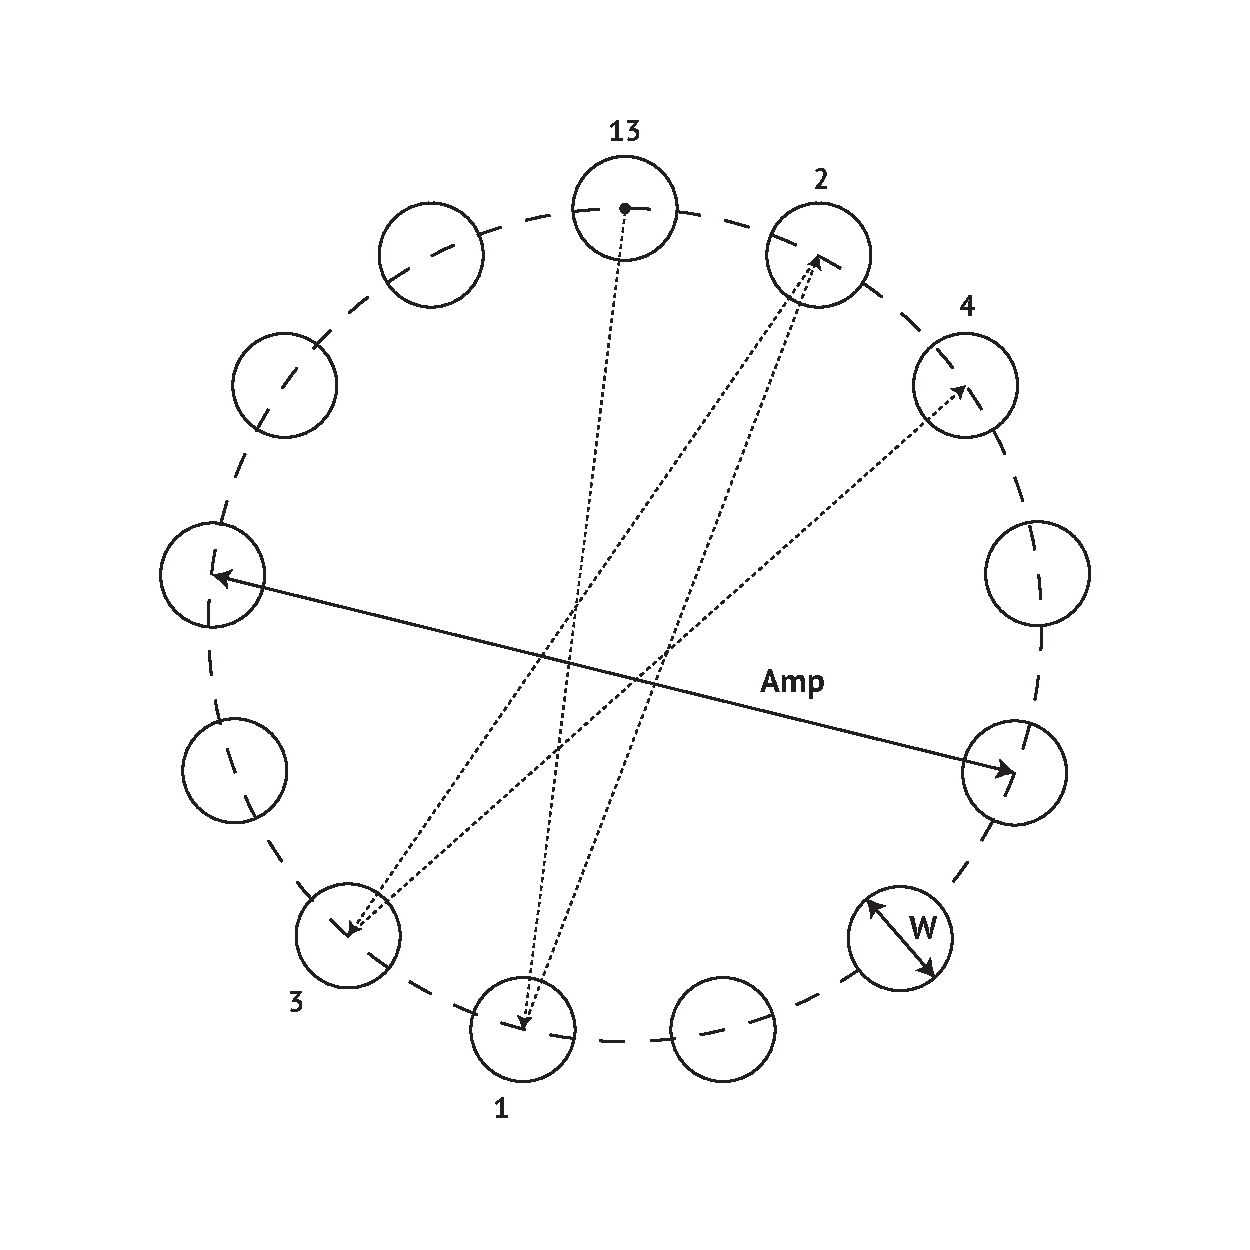
\includegraphics[width=.7\columnwidth]{graphics/fitts_law_circle.pdf}
    \caption{Multidirectional pointing \& clicking task}
    \label{fig:pointing_task}
\end{figure}

\subsection{Study implementation}

On the basis of the previous discussions, the software was implemented to run the study with participants. There are 8 rounds (2 body positions, 2 arm positions, 2 degrees of freedom = 8 possibilities) for each participant, which differ in the following modes:

\begin{table}[h]
    \centering
    \begin{tabular}{|p{5cm}||p{3cm}|p{3cm}|}
    \hline
    arm position & stretched out & applied to the body \\
    participants position & standing & sitting \\
    controller degree of freedom & 3 & 6 \\
    \hline
    \end{tabular}
    \caption{Task modes}
    \label{tab:task_modes}
\end{table}

Each of these rounds contained six Fitts' Law circles, based on the six different \textit{ID} values for width and amplitude calculated in Table~\ref{tab:id_values}. The modes mentioned in~\ref{tab:task_modes} and the previously mentioned circles were combined with the help of Latin Squares. These Latin Squares were used to give each participant a different sequence of modes and of circles. The implementation calculated the two of these Latin Squares. One to iterate through the different possible combinations of arm position, body position and degrees of freedom. The other one was used to iterate through the possible amplitudes and sizes of the Fitts' Law circle task. Both are based on a unique user id, so the iterations are steady.

\subsection{Design}
\label{subsec:design}

Resulting from the previous research and testing, the experiment had five different and independent variables in a 2 x 3 x 2 x 2 x 2 arrangement (makes a total of 48 combinations):

\begin{itemize}
    \item Target amplitude: 350 and 150;
    \item Target width: 15, 30 and 50;
    \item Arm position: stretched out and applied to body;
    \item User position: standing and sitting;
    \item Degrees of freedom: 6 and 3;
\end{itemize}

Based on these numbers, each participant had to complete 48 Fitts' Law circles with each 13 recorded targets and two clicks each target. Given the 16 subject participating of this study, it results in a total number of $16 \cdot 48 \cdot 13 \cdot 2 = 19,968$ trials.

\subsection{Tracking device jitter}
\label{subsec:basic_jitter}

To eliminated device jitter, the position of the controller and headset were tracked in a total static position (headset on a table and controller on the floor). The controller and headset showed fluctuations in position, even when in a total static position. The results were used in Subsection~\ref{subsec:evaluation:clearing_the_data:device_caused_jitter} to clear the data from the device-caused jitter.

\subsection{Source Code}
\label{subsec:source_code}

The full source code and all assets can be found in a GitHub repository\footnote{\url{https://github.com/mc17uulm/Heisenberg}}. Under $assets/HeisenbergScene/Scripts$ all relevant scripts can be found. The script $Processing.cs$ is the entry point for the application.

\section{Experiment}
\label{sec:experiment}

\subsection{Participants}
\label{subsec:participants}

All of the sixteen participating subjects were actual or former students of the Ulm University. The ages of the participants reached from 20 to 30 years (by an average age of 24.5 years). The group of participants consisted of into 8 male, 7 female, and one other. 15 out of 16 subjects were right-handed. 7 out of 16 had visual aids.

Most of them had already experience with virtual reality: 13 of 16 participants used VR at least once, 11 out of 16 had even more than one month of experience in VR. Half of the subjects used VR frequently. The subject also got asked if they ever used games in VR, where pointing and shooting is the main task. Half of the subjects reported so. When to judge their skills, the subjects reported an average value of 2.5 (by a scale from 1 to 5; 1 is basic and 5 is skilled). 

The duration of the study was 40 minutes to one hour, mostly based on the pointing skills and strategies of the participants. 

\begin{figure}[h]
    \centering
    \subfigure[User is standing with stretched out  arm]{{\includegraphics[width=.4\linewidth]{graphics/standing.pdf}}}
    \qquad
    \subfigure[User is sitting with stretched out arm]{{\includegraphics[width=.4\linewidth]{graphics/sitting.pdf}}}
    \caption{Body positions in study}
    \label{fig:body_positions}
\end{figure}

\subsection{Procedure}
\label{subsec:procedure}

The user held the controller in his dominant hand and was able to interact via a click on the trigger. After the user read the task (Task description illustrated by Figure~\ref{fig:procedure-design} (c)) and changed his arm and/or body position he could start the round by clicking the trigger. By starting a round, all controller positions, rotations, and clicks were tracked and logged. Between these rounds, the user had the change to have a small break and rest his arm.

Each of these eight rounds showed one target at a time. The user had to direct his controller to the target (the user could see where he was pointing by a raycast) and click for the first time. This click was called the ``ballistic click'' because it resulted out of the motion. It wasn't necessary for the click to be on target. The data should show where the user aimed to and where he finally ended when clicking the trigger. For the second click, the user had to be on target for at least 500 milliseconds (illustrated by a timer turning from red to green - example in Figure~\ref{fig:procedure-design} a \& b). This second click was called ``static click``. The click in this position was necessary to compare the differences between a click out of motion and one out of a static pointing on the target. 

All targets were placed on a circle, which implemented a standard Fitts' task. But only the actual target was shown to the user. After the two clicks on one target, the next target was shown.

\begin{figure}[h]
    \centering
    \subfigure[Timer is running]{{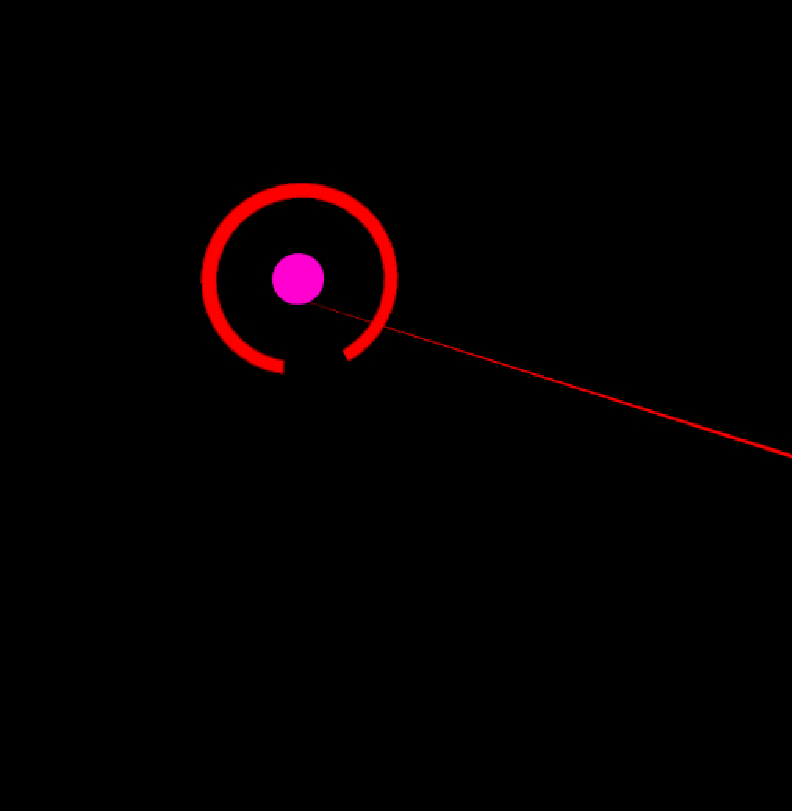
\includegraphics[width=.25\linewidth]{graphics/in_app_graphics/heisenberg_final_click_filling_small.pdf}}}
    \qquad
    \subfigure[Timer is finished and user has to click]{{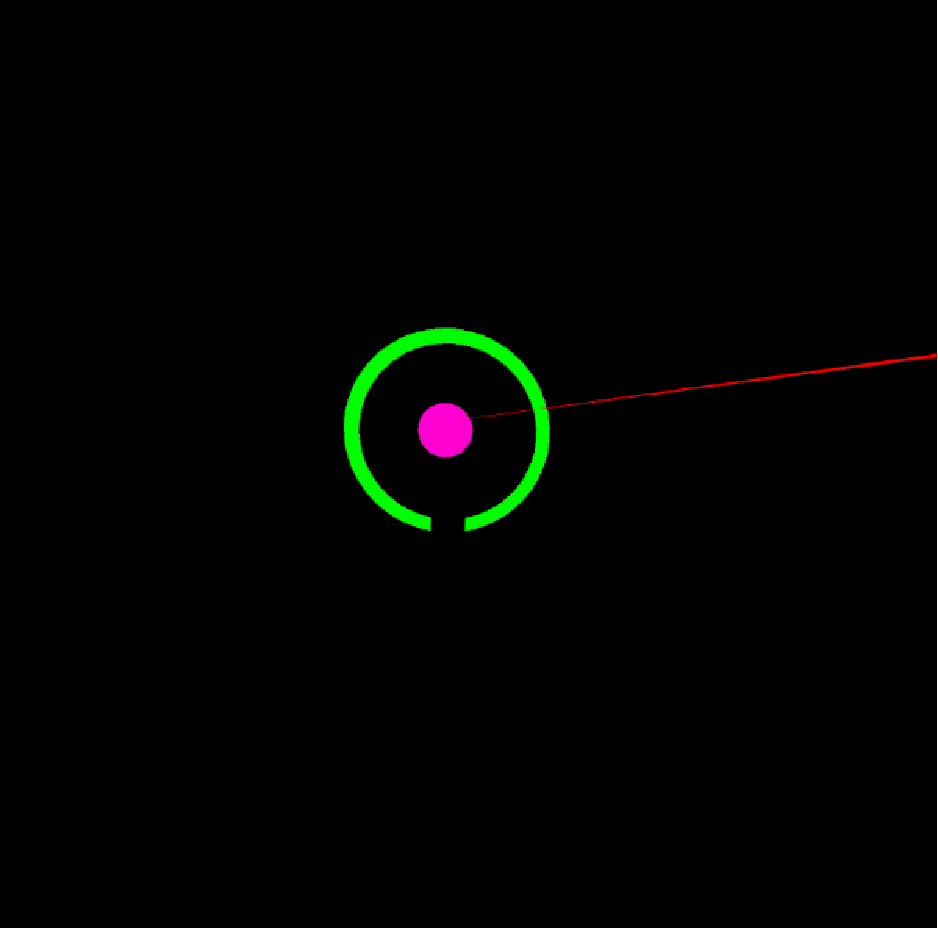
\includegraphics[width=.25\linewidth]{graphics/in_app_graphics/heisenberg_final_click_filled_small.pdf}}}
    \qquad
    \subfigure[New task is shown to the user. In between these tasks the user could rest]{{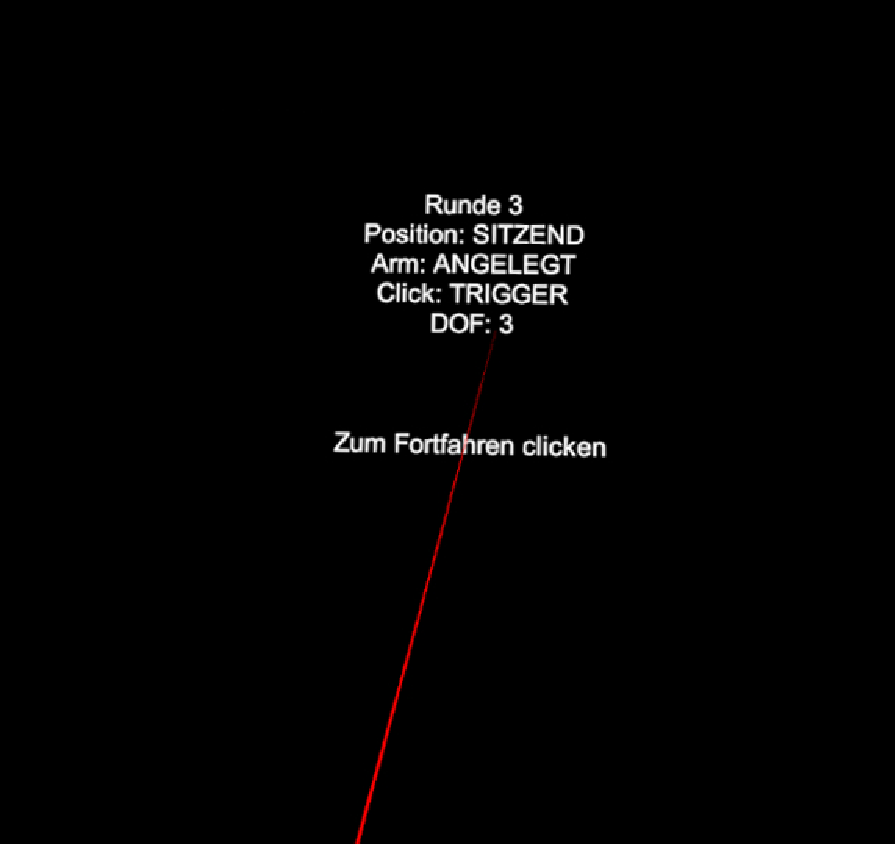
\includegraphics[width=.25\linewidth]{graphics/in_app_graphics/heisenberg_final_task_small.pdf}}}
    \caption{Procedure in real application}
    \label{fig:procedure-design}
\end{figure}

\section{Collected Data}
\label{sec:results}

The software saved all tracked data in csv files (\textbf{c}haracter \textbf{s}eperated \textbf{v}alues) for each user. Following values get tracked:

\begin{itemize}
    \item Identification of the user (only an id to match with the demographic data)
    \item Standard information about the task (arm and body position; degrees of freedom; a timestamp)
    \item Events and system states (pressed trigger, click, etc.)
    \item Strength of pressure on the trigger (value between 0 and 1)
    \item Position and size of the target
    \item Position and rotation of the controller
    \item Position of pointer on canvas
\end{itemize}

These values were tracked and saved for each frame. To ease the evaluation of the data (all of the tracked data for one participant ranged from 20 megabytes (MB) to 45 MB.), the software produced two extra log files. In one of them, the point of first press and click were selected and the difference between them calculated and saved. In the other one, the software saved the calculated \textit{Throughput} and the values (\textit{Effective Width}, \textit{Effective Distance}, \textit{Effective ID}, \textit{Effective Throughput} and \textit{Mean Movement Time}) based on the model of the Extended Fitt's Law, explained in Section~\ref{subsec:related-work:background:extended_fitts_law}. So each trial with on participant ended with three anonymous log files.


%% evaluation.tex
%%

%% ==============================
\chapter{Results}
\label{ch:results}
%% ==============================

To find indications for the ``Heisenberg Effect'' in the collected data, it was important to first take a look at other effects that may occur and had an influence on the accuracy of the pointing tasks. The paper done by Pavlovych and Stuerzlinger~\cite{pavlovych_tradeoff_2009} suggest to take a deeper look on hand tremor and device jitter to precisely analyze effects in distal pointing tasks. 

\section{Clearing the data from disturbing effects}
\label{sec:evaluation:clearing_the_data}

\begin{figure}[h]
    \centering
    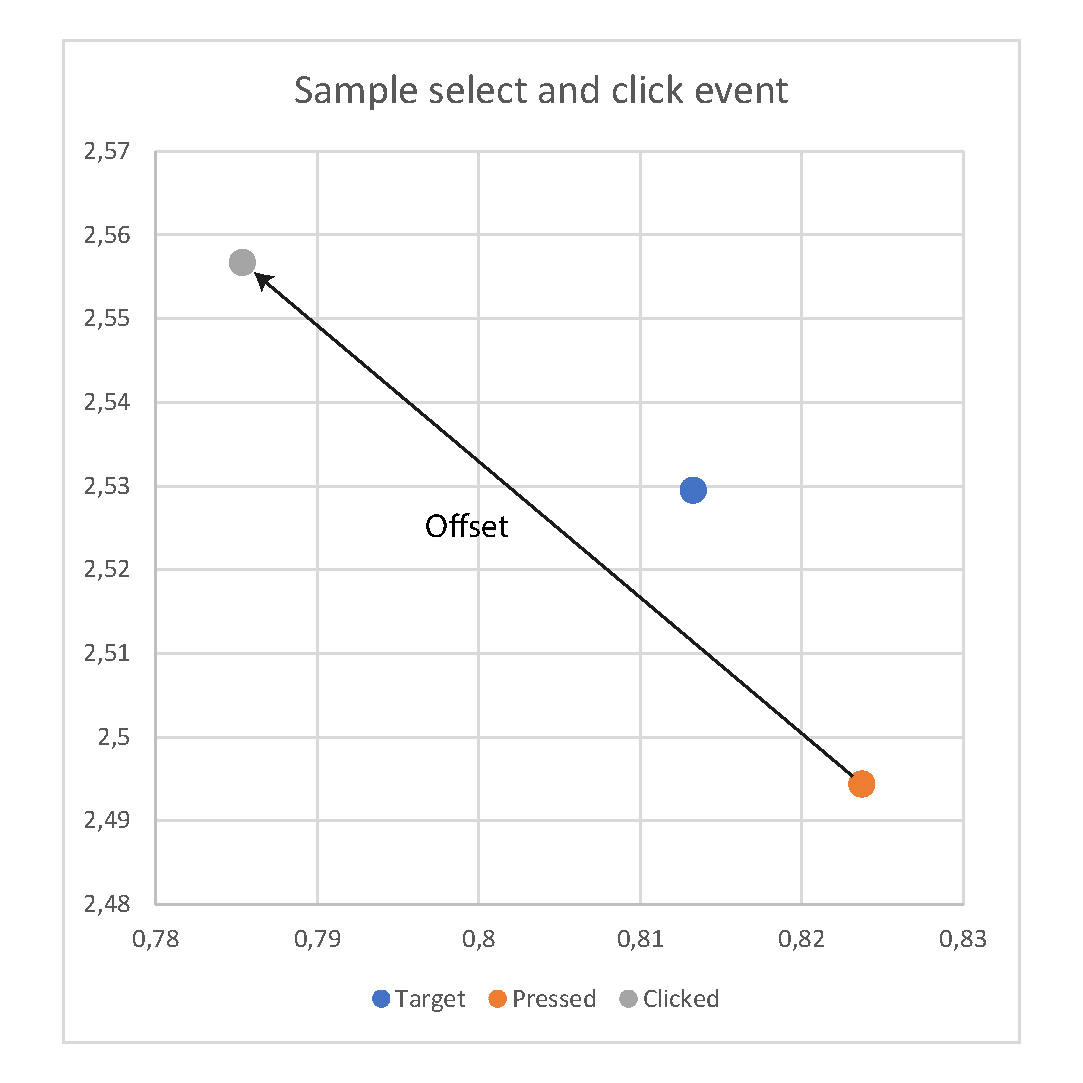
\includegraphics[width=.45\columnwidth]{graphics/graphs/sample_point_and_click_event_edited.pdf}
    \caption{A single sample from the data. }
    \label{fig:sample_point_and_click_event}
\end{figure}

\subsection{Calculation offset}
\label{subsec:evaluation:clearing_the_data:calculating_offset}

To clear the data from disturbing effects, it was important to analyze the overall offset at first. With offset, it is meant the distance between the position of the cursor, where the user first slightly pressed the trigger (a slight press is not activating a click event. The trigger has to be fully pressed in), and the position of the cursor, when the user clicked and hit the target. It was to suspect, that in this offset, the ``Heisenberg Effect'' can be found. For illustration, Figure~\ref{fig:sample_point_and_click_event} shows in orange the position when the user first pressed the trigger. The blue dot marks the actual target and the grey dot marks the position where the controller pointed at when the user fully clicked the trigger. The distance between the pressed position and the clicked position is the described offset.

\subsection{Device-caused jitter}
\label{subsec:evaluation:clearing_the_data:device_caused_jitter}

As mentioned in Subsection~\ref{subsec:basic_jitter}, the jitter caused by the controller and the VR headset were tracked while both devices weren't moved at all. The controller was placed on the floor and the headset on a table. The tracked positions showed a small fluctuation in the position reporting of the devices. With the saved positions a maximum and minimum of these fluctuations were calculated and set in perspective with the other effects. In Figure~\ref{fig:static_device_jitter_compared_to_offset} is shown how minimal the effect of the jitter based on the devices is, compared to the overall offset. The offset is in this figure, the difference between the point the user is first pressing the button to select a target, and the position the click event is tracked.

\begin{figure}[h]
    \centering
    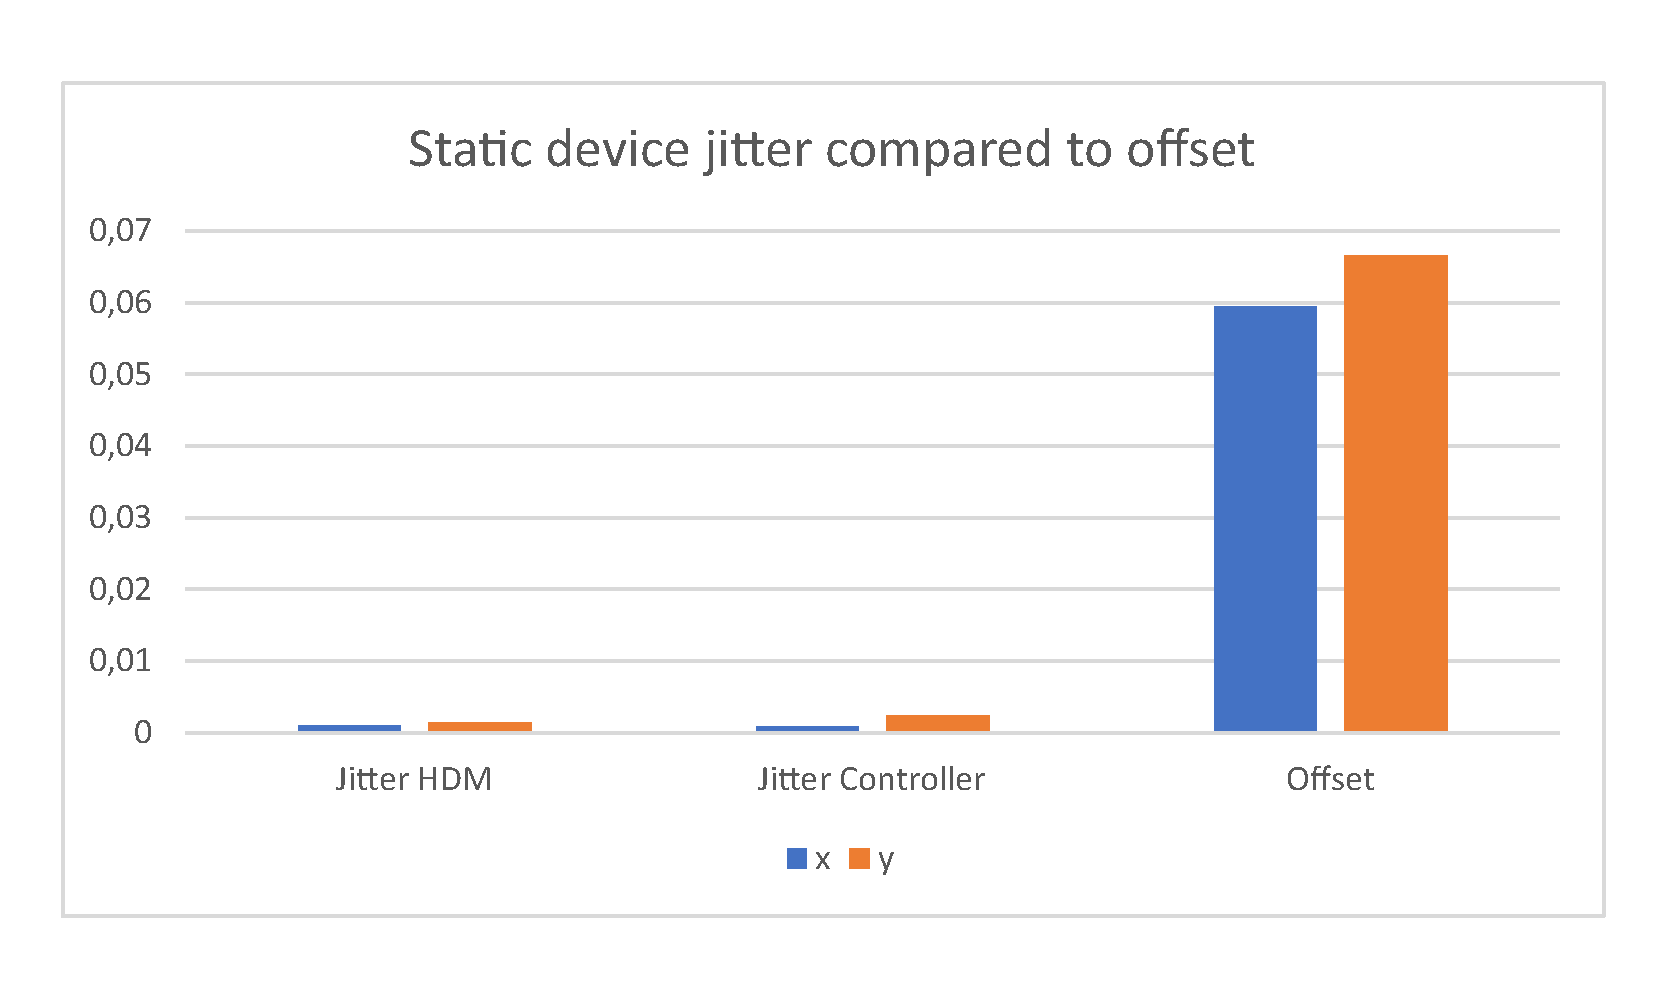
\includegraphics[width=.9\columnwidth]{graphics/graphs/static_device_jitter_compared_to_offset.pdf}
    \caption{Static jitter of the devices compared to the actual offset between intention to click and result hit on the target}
    \label{fig:static_device_jitter_compared_to_offset}
\end{figure}

\subsection{Hand tremor}
\label{subsec:evaluation:clearing_the_data:hand_tremor}

To determine the effects of hand tremor to the data, the changes in position were tracked, when users had to hold still in the target for finishing the timer. These fluctuations were plotted over all tasks. Tasks are here the different stages of the procedure: to stand up/sit down, to stretch the arm out/apply it to the body and the degrees of freedom given to the controller. The data for the offset was also distributed over these tasks and set in comparison to the data calculated as the hand jitter. The result is shown in Figure~\ref{fig:difference_handjitter_offset}. The figure shows clearly, that hand tremor has an impact on the accuracy of the pointing but can't be declared as the main reason for the offset. It is also shown, that with the arm stretched out hand tremor increases as expected.  

\begin{figure}[h]
    \centering
    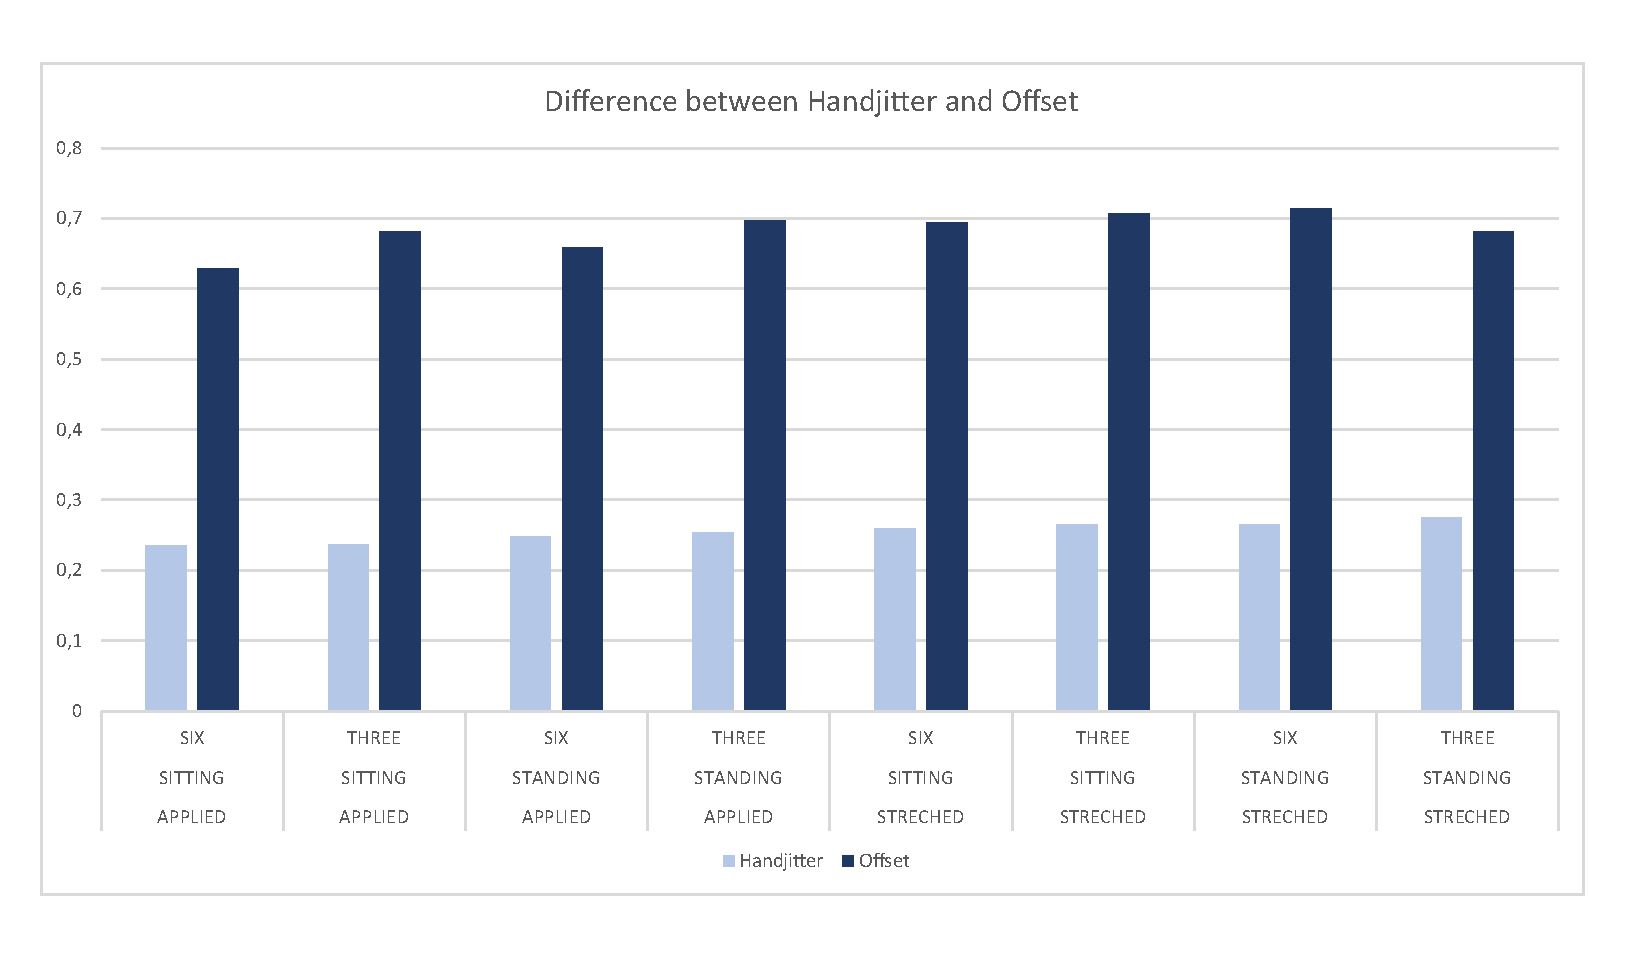
\includegraphics[width=.9\columnwidth]{graphics/graphs/difference_handjitter_offset.pdf}
    \caption{Difference between offset by hand tremor and overall offset plotted over all different tasks}
    \label{fig:difference_handjitter_offset}
\end{figure}

\section{Indications for the Heisenberg Effect}
\label{sec:evaluation:indications}

\begin{figure}[h]
    \centering
    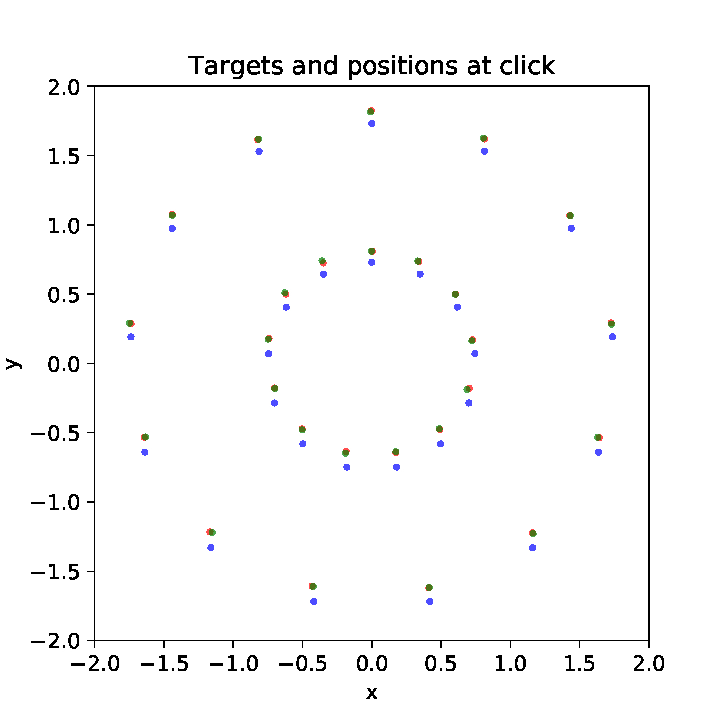
\includegraphics[width=.75\columnwidth]{graphics/graphs/final_plot.pdf}
    \caption{Combination of all targets and results}
    \label{fig:plot}
\end{figure}

After clearing the data and setting it in comparison with other effects, it is clear, that hand tremor and device jitter aren't the main reasons for the offset between aimed position and hit position in the collected data. The results suggest, that the, first by Bowman~\cite{bowman_using_2001} mentioned, ``Heisenberg Effect'' is the reason for this offset. 
\newline
\newline
If all data is plotted together, the effect gets even clearer. A look at Figure~\ref{fig:plot} shows, that the offset has one direction, upwards. The blue dots symbolize the targets on the Fitt's Law based circle (as explained in detail in subsection~\ref{subsec:impl:circle_task}), and the green and red dots symbolize the final position of the hit, when the click was tracked (green are the positions with 3DOF and red are the positions with 6DOF). Hand tremor and device jitter would have caused balanced ``hit fields'' around the targets. The collected data suggest, that the effects of hand tremor and jitter result in a normal distribution around the targets. But as the Figure shows, all hits are above the target. This suggests the conclusion, that the up going movement of the click, is resulting in this offset. 
%% conclusion.tex
%%

%% ==============================
\chapter{Conclusions and future work}
\label{ch:conclusion}
%% ==============================

\section{The ``Heisenberg Effect''}
\label{sec:conclusion:heisenberg}

The analysis of the collected data in section~\ref{sec:evaluation:indications} shows that there is an effect, which cannot be explained by hand tremor or device jitter, resulting in a worse pointing accuracy and maybe even a worse throughput. This effect shows many similarities to the described ``Heisenberg Effect'' by Bowman~\cite{bowman_using_2001} and Kopper et al.~\cite{kopper_human_2010}, like the occured offset in direction of the pressed trigger, demonstrated in Figure~\ref{fig:plot}. 

The incentive to this work was to show evidence for the ``Heisenberg Effect'', analyze its effects and give a good basis for compensating it. The results which are shown in this thesis leap to the conclusion, that the ``Heisenberg Effect'' exists and has a bigger impact on pointing accuracy and throughput as previously thought.

\section{Compensation for the ``Heisenberg Effect'' and Implications for future work}
\label{sec:conclusion:compensation_future_work}

\begin{figure}[h]
    \centering
    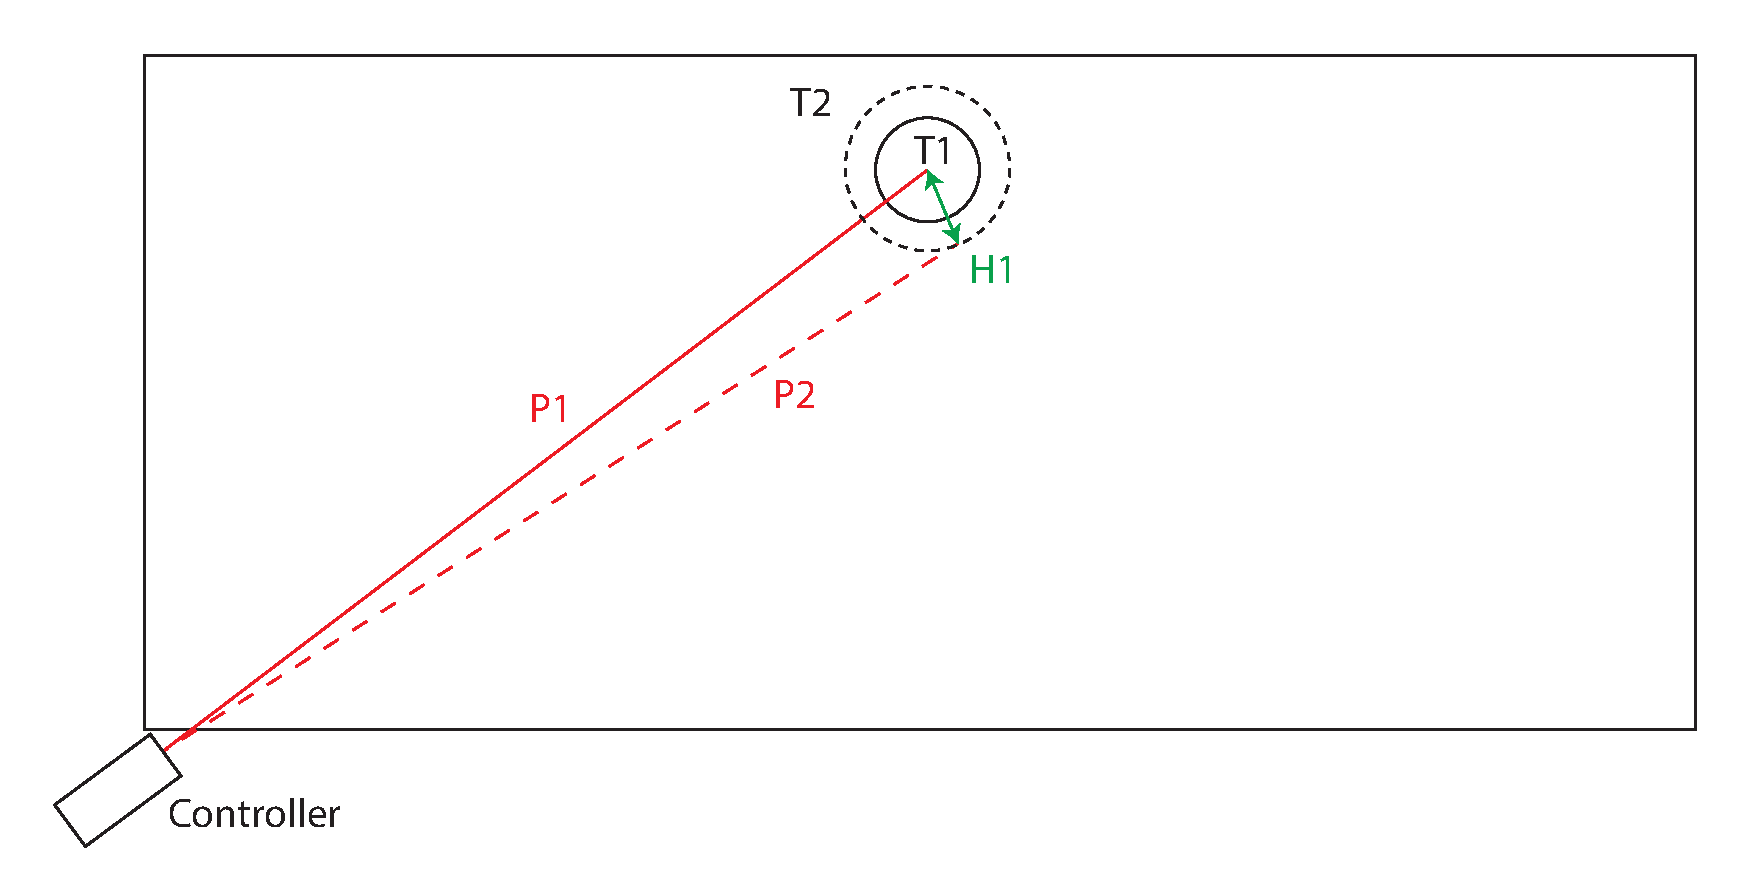
\includegraphics[width=.7\columnwidth]{graphics/heisenberg_effect_compensated.pdf}
    \caption{Possible Compensation for the Heisenberg Effect}
    \label{fig:heisenberg_effect_compensated}
\end{figure}

Because the ``Heisenberg Effect'' shows a similar range of effect on different modalities (like shown in Figure~\ref{fig:difference_handjitter_offset}), there is a chance, this effect can be predicted and measured. If this is, in an efficient algorithm and time possible, the effect could be canceled out in real life applications. For future work, it would be interesting to analyze the ``Heisenberg Effect'' in more real-life applications. A possible way to implement this, was already given by MacKenzie in his work on an extended Fitt's Law (described in subsection~\ref{subsec:related-work:background:extended_fitts_law})~\cite{mackenzie_extending_1992}: With enough data, it is possible to calculate if the user \textbf{wanted} to hit the target, more than if he really did. The software could now count a target as clicked on or hit, even if the user didn't hit it directly. Future work would have to take in consideration, that the created lag, caused by this additional computing time, could also have an effect on the performance of the user, like suggested by Pavlovych and Stuerzlinger~\cite{pavlovych_tradeoff_2009}.

The Figure~\ref{fig:heisenberg_effect_compensated} shows such a possible situation. The user wants to click on the target (T1) and aims the controller on this target (Line P1). Based on the disturbance in pointing made through the click (Line P2), the system would not detect this click, as one in the target. Because the ``Heisenberg Effect'' can be plotted over time, the system could now detect, that the user wanted to hit a target, a little bigger than the actual target (bigger target labeled as T2). Now the click is in the expanded target and the click would count.

One problem with the ``Heisenberg Effect'' wasn't cleared already and could be a topic for future work: The decrease of pointing accuracy could have an effect on the throughput. This aspect of the ``Heisenberg Effect'' wasn't discussed in this work. To sum up this work: it is clear that the effect needs to be farther researched, but a good base is given here.

\section{Acknowledgements}
Special thanks to Dennis Wolf for his help and advice in creating this thesis. 

%\appendix
%% %% appendix.tex
%%
\appendix

%% ==============================
\iflanguage{ngerman}{\chapter{Anhang}}{\chapter{Appendix}}
\label{ch:appendix}
%% ==============================


\backmatter %%%%%%%%%%%%%%%%%%%%%%%%%%%%%%%%%%%%%%%%%%%%%%%%%%%%%%%%%%%%%%%%%%

\listoffigures
\listoftables

%\bibliographystyle{natdin}
\bibliographystyle{IEEEtranS}	% alternativer Stil
\bibliography{bibliography} % Bib-Datei

\cleardoublepage
\clearscrheadfoot
\declaration

\end{document}
